\documentclass[letterpaper, landscape]{exam}
\usepackage{2in1, lscape} 
\printanswers

\usepackage{units} 
\usepackage[fleqn]{amsmath}
\usepackage{float}
\usepackage{mdwlist}
\usepackage{booktabs}
\usepackage{caption}
\usepackage{fullpage}
\usepackage{enumerate}
\usepackage{graphicx}
\usepackage{xfrac}

\setcounter{tocdepth}{1}
\everymath{\displaystyle}

\author{}
\date{\today}
\title{Calculus I \\ Week Two}

\begin{document}

  \maketitle
  \tableofcontents

  \section{Velocity}

  \begin{itemize*}
    \item draw graph of projectile motion
    \item show average velocity is slope of secant line
    \item show how secant line approaches tangent line as points get closer
      together
    \item describe instantaneous velocity as slope of tangent line
    \item do some problems from exercises
  \end{itemize*}

  \section{Limits}

  \subsection{Zeno}
  \begin{itemize*}
    \item Describe Zeno's paradox with arrow
    \item Show how area of square is: 
      \[
        \sum_{x = 1}^\infty \frac{1}{2^x}
      \]

    \item The limit is the number you get closer and closer to without
      necessarily ever reaching.

    \item You can get as close as you want to 1 by adding more terms, but you
      never get to 1.

  \end{itemize*}

  \subsection{Informal Definition}

  \[
    \lim_{x \to a} f(x) = L
  \]

  \begin{itemize*}
    \item You can make $f(x)$ as close as you want to $L$ by taking values suitably
      close to $a$
    \item Value of $f(a)$ doesn't matter
    \item $f(a)$ doesn't have to be defined
  \end{itemize*}

  \subsection{Numeric Examples}

  \subsubsection{Example 1}
  \[
    \lim_{x \to 0} \frac{\sin x}{x} = 1
  \]

  Review definition of sine and draw graph.

  \begin{tabular}[H]{rr}
    \toprule
    x     & $f(x)$ \\
    \midrule
    -1    & 0.841471 \\
    -0.5  & 0.958851 \\
    -0.1  & 0.998334 \\
    -0.05 & 0.999583 \\
    -0.01 & 0.999983 \\
    0.01  & 0.999983 \\
    0.05  & 0.999583 \\
    0.1   & 0.998334 \\
    0.5   & 0.958851 \\
    1     & 0.841471 \\
    \bottomrule
  \end{tabular}

  \begin{itemize*}
    \item note that $f$ is not defined for $x = 0$
    \item Review definition of sine and draw graph.
    \item note that graph of numerator ($\sin x$) looks like graph of $y = x$ around zero
  \end{itemize*}

  \begin{figure}[H]
    \centering
    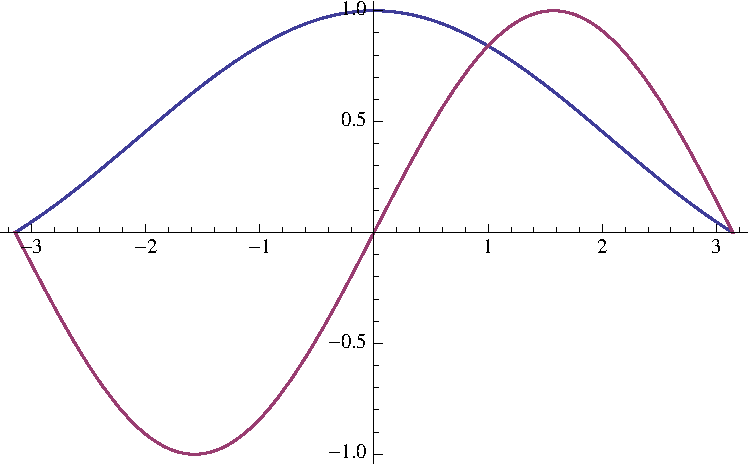
\includegraphics[scale = 0.5]{example1.pdf}
    \caption{$\sin x$ and limit}
    \label{fig:example1}
  \end{figure}

  \subsubsection{Example 2}
  \[
    \lim_{x \to 0} \frac{1 - \cos x}{x} = 0
  \]

  \begin{itemize*}
    \item note that $f$ is not defined for $x = 0$
    \item Review definition of cosine and draw graph.
    \item note that graph of numerator ($1 - \cos x$) looks like graph of $y =
      0$ around zero
  \end{itemize*}

  \begin{tabular}[H]{rr}
    \toprule
    x     & $f(x)$ \\
    \midrule
    -1    & -0.459698 \\
    -0.5  & -0.244835 \\
    -0.1  & -0.0499583 \\
    -0.05 & -0.0249948 \\
    -0.01 & -0.00499996 \\
    0.01  & 0.00499996 \\
    0.05  & 0.0249948 \\
    0.1   & 0.0499583 \\
    0.5   & 0.244835 \\
    1     & 0.459698 \\
    \bottomrule
  \end{tabular}

  \begin{figure}[H]
    \centering
    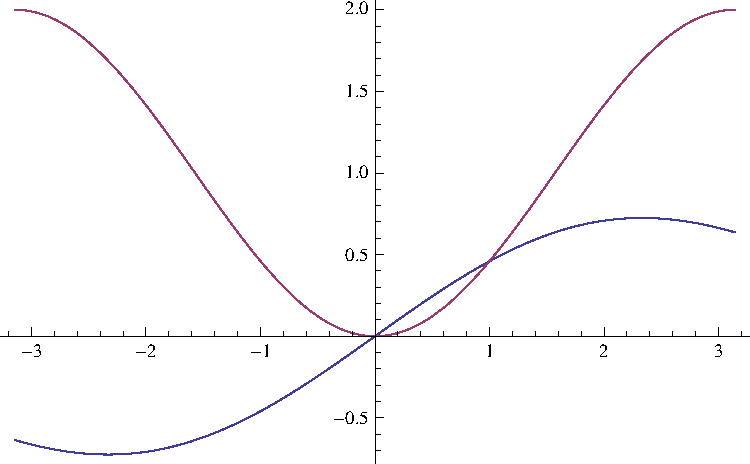
\includegraphics[scale = 0.5]{example2.pdf}
    \caption{$1 - \cos x$ and limit}
    \label{fig:example2}
  \end{figure}

  \section{Graphic Examples}

  Draw graph of:
  \begin{itemize*}
    \item $f(a)$ not defined
    \item $f(a) \neq \lim_{x \to a} f(x)$
  \end{itemize*}

  \section{Rational Function Example}

  \begin{enumerate}
    \item 
      \begin{align*}
        f(x) & = \frac{x^2 + 5x + 9}{x + 3} \\
             & = \frac{(x + 2)(x + 3)}{x + 3} \\
             & = x + 2 \\
             \\
        \lim_{x \to -3} f(x) &= -1 \\
      \end{align*}

      Show that limit is the same even if you define a piecewise function with
      $f(x)$ defined to be any value.

    \item $\lim_{x \to -1^-} \frac{x + 3}{x + 1} = -\infty$

    \item $\lim_{x \to -1^+} \frac{x + 3}{x + 1} = \infty$

  \end{enumerate}

  \section{One-Sided Limits}

  \[
    f(x) = \frac{|x|}{x}
  \]

  \begin{itemize}
    \item draw graph
    \item $\lim_{x \to 0^-} f(x) = -1$
    \item $\lim_{x \to 0^+} f(x) = 1$
    \item $f(0)$ is not defined
  \end{itemize}

  \begin{itemize}
    \item Draw other examples of graphs with one sided limits.
    \item The overall limit is only defined if the left and right limits are
      equal
  \end{itemize}

  \section{Infinite Limits}
  \begin{itemize}
    \item $\lim_{x \to a} = \pm \infty$
    \item left and right limits
  \end{itemize}

  \begin{itemize}
    \item $f(x) = \frac{1}{x}$
    \item $f(x) = \frac{2x + 1}{x - 1}$
  \end{itemize}

  Describe equations of vertical asymptotes.

  \section{Find Function}

  Draw the graph of a function that satisfies:
  \begin{itemize}
    \item $\lim_{x \to 1^-} f(x) =  3$
    \item $\lim_{x \to 1^+} f(x) =  -2$
    \item $f(1) = 2$
    \item $\lim_{x \to -1^+} f(x) = -\infty$
    \item $\lim_{x \to -1^-} f(x) = \infty$
  \end{itemize}

  \section{Logarithms}
  \[
    a = \log x \rightarrow 10^a = x
  \]

  \begin{itemize*}
    \item $\log 0$ is not defined because there isn't any number where
      $10^a = 0$
    \item range of $\log$ is positive numbers
    \item as $x$ gets smaller and smaller, $\log x$ gets more and more negative
  \end{itemize*}

  \[
    \lim{x \to 0} \log x = -\infty
  \]

  draw graph

  \section{Tangent}

  \begin{itemize*}
    \item draw picture of circle with tangent line
    \item show where tangent function comes from
    \item show how as angle goes from 0 to $\sfrac{\pi}{2}$ 
      $\tan x \rightarrow \infty$
    \item show how as angle goes from 0 to $- \sfrac{\pi}{2}$ 
      $\tan x \rightarrow -\infty$
  \end{itemize*}

  \section{Theory of Relativity}

  \[
    m = \frac{m_0}{\sqrt{1 - \frac{v^2}{c^2}}}
  \]

  Nothing can go faster than the speed of light. The cosmic speed limit is
  enforced by the increase in mass as things go faster.

  \begin{align*}
    a(m)                     & = \frac{F}{m} \\
    \lim_{m \to \infty} a(m) & = 0 \\
  \end{align*}

  \begin{itemize*}
    \item a given force produces less and less acceleration as the velocity
      increases
    \item as the mass approaches infinity the acceleration approaches zero
  \end{itemize*}

\end{document}

